\documentclass[11pt]{article}
\usepackage[margin=1in]{geometry}
\usepackage{amsmath}
\usepackage{amsthm}
\usepackage{fontspec}
\usepackage{unicode-math}
\setmathfont{latinmodern-math.otf}
\usepackage{booktabs}
\usepackage{longtable}
\usepackage{array}
\usepackage{graphicx}
\usepackage{microtype}
\usepackage[table,dvipsnames]{xcolor}
\usepackage{tikz}
\usetikzlibrary{arrows.meta,positioning,fit,backgrounds}
\usepackage{enumitem}
\usepackage{caption}
\captionsetup{font=small,labelfont=bf}
\usepackage[hidelinks,breaklinks]{hyperref}

% --- theorem environments (match the conversion spec) ---
\theoremstyle{plain}
\newtheorem{lemma}{Lemma}
\newtheorem*{thmTtwo}{Theorem T2}
\newtheorem*{corTtwop}{Corollary T2$'$}
\theoremstyle{definition}
\newtheorem*{mydef}{Definition}

\setlength{\parskip}{0.35em}
\setlist{nosep,leftmargin=1.4em}
\hyphenpenalty=2000

\title{\bfseries The Readout Regime:\\ A Normal Form for Final-Residual Control of Frozen Transformers\\ --- and Its Capacity Limits}
\author{Nathan Lee Peterson\\[2pt]
  \normalsize Independent researcher\\
  \normalsize Correspondence: \texttt{orbitnate@gmail.com}\\
  \normalsize Code and result artifacts: \url{https://github.com/orbitnate/readout-regime}}
\date{}

\begin{document}
\maketitle


\begin{abstract}
Inference-time interventions on a frozen transformer --- steering behavior, injecting facts, suppressing outputs --- are not interchangeable: \emph{where} an additive intervention acts splits them into two regimes of sharply different expressive power, and we give the exact theory of one. An intervention that writes into the \textbf{final residual stream} (the unembedding/readout space; installing a scaled row of the output-projection matrix \texttt{lm\_head} is the exactly-characterizable case) induces on the next-token logits, for every input, the transform $z \mapsto s(x)\cdot z + c(x)$: a ranking-preserving scalar temperature $s(x) > 0$ plus a re-ranking bias $c(x)$ \textbf{confined to a fixed, low-dimensional set of directions chosen before any input is seen} (T1; verified against direct forward-pass computation to $\approx 5\times10^{-6}$). The result that matters is a \emph{structure} theorem (T2): the input selects only a \emph{point} in that fixed set and a temperature, so the reachable re-ranking directions, over all inputs, have affine dimension at most the installed-slot count. \textbf{In plain terms: a readout install can re-weight and re-rank the options the model already has, but cannot synthesize a new answer direction or compute a hidden routing variable the addressing query does not already expose.} We prove the readout regime's confinement and \emph{cite} --- not prove --- evidence that the representation regime is not so confined; that direct measurement is the main open item. The corollaries, carefully bounded: a bounded readout install is \textbf{not a hard override} of a peaked prior, can only \textbf{tip} a decision the context has already scaffolded near-balanced, and \textbf{cannot compute} a hidden intermediate. Capacity has two faces, both empirical: across \textbf{key-disjoint} decisions installs compose bit-exactly at scale (tens of modules, thousands of facts, $\Delta=0$); \textbf{within one} decision the readout is winner-take-all ($\approx 2$ targets co-winnable, against an output projection of entropy-effective rank $\approx 918$). The control reading: \emph{tip} a propensity in the readout regime --- it is auditable, a removable bias --- but place any hard guarantee in a deterministic override outside the model. The contribution is the boundary, stated precisely.
\end{abstract}

\section{Introduction}

A growing toolbox modifies a frozen language model at inference time rather than by fine-tuning: activation/representation steering, function vectors, knowledge editors, attention-injected memories, and logit-space biases. These methods are attractive precisely because they are cheap, removable, and leave the base weights untouched. But they are not interchangeable, and the literature has not drawn a clean line between what each \emph{can} and \emph{cannot} do.

This paper draws that line for the case where the intervention is \textbf{additive in the final residual stream}: a vector added to the hidden state at the current decoding position, whose effect reaches the unembedding through the model's final normalization with no further nonlinear processing. The most exact instance --- and our analytic anchor --- is installing a scaled \textbf{row of the output-projection matrix} (\texttt{lm\_head}), the ``value = unembedding row of a target token'' construction. That \texttt{lm\_head} rows are special directions in this space is not new: the observation that ``row \emph{i} of \texttt{lm\_head} is precisely the direction that produces high probability for token \emph{i}'' appears in recent work on retrofitting memory to frozen models (Wind, 2026, \S4.4.3; see \S8). We do not claim that observation. We claim its consequences, and we prove them.

\textbf{Contributions.}

\begin{enumerate}
\item \textbf{T1 --- exact readout transform (known core; exact form).} A final-residual additive install induces, on the next-token logits, the transform $\tilde z(x) = s(x)\cdot z(x) + c(x)$, where under RMSNorm $s(x) = r/r^{\prime} > 0$ is a scalar temperature and $c(x)$ is a combination of \textbf{fixed} directions $u_t = U(\gamma \odot U[t])$. The no-norm case is the exact additive Gram-column bias $\tilde z = z + \alpha\cdot U U[t]$; the LayerNorm case folds in a fixed centering (Lemma 4). We verify the closed form numerically against direct forward-pass computation to max-diff $4.77\times10^{-6}$ (Mistral-7B) and $7.15\times10^{-6}$ (Qwen2.5-7B).

\item \textbf{T2 --- cone-confinement structure theorem (the contribution).} Across \textbf{all} inputs, a readout install's re-ranking term $c(x)$ lies in a single \textbf{fixed} set $C$ of affine dimension $\le m$ (the slot count) --- the convex cone generated by the installed (possibly signed) generators --- chosen before any input. The input selects only a \emph{point} in $C$ (via key-addressed weights) and a temperature. Hence the reachable set of re-ranking directions, over all inputs, has rank $\le m$, and a readout install \textbf{cannot synthesize a re-ranking direction outside the pre-installed set} (defined precisely in \S4.3). This holds \emph{even with} input-conditional, key-addressed attention over an arbitrary stored set, and uses only that the stored values are fixed before input and the weights are non-negative --- \emph{not} the \texttt{lm\_head} identity (which is what makes T1 exact, \S2 remark). The unconditional, $m$-independent content is \textbf{fixedness} (no input creates a re-ranking direction outside the $m$ pre-stored generators); the $\textit{rank} \le m$ \emph{number} bites only when $m$ is small relative to the answer cardinality --- it is vacuous once $m$ approaches the output projection's $\approx918$ effective rank. (T2(a)--(c) follow from Lemmas 1/3/4; the load-bearing novelty is this fixedness/capacity statement and its measurable form, Corollary T2$^{\prime}$, not the per-input algebra.)

\item \textbf{Corollaries (operational, carefully bounded).} T2 implies a readout install (C1) gives \textbf{no hard override} of a peaked prior --- a bounded install flips a decision only when its fixed-cone correction beats the scaled base gap; (C2) can \emph{tip} a context-scaffolded near-balanced decision; and (C3) cannot \emph{compute or synthesize} a hidden routing variable or a new answer direction --- it can exploit a hidden intermediate only insofar as the addressing query already exposes it. Each is a bounded consequence, not a sweeping impossibility.

\item \textbf{Capacity observations (empirical, not a theorem).} Across \textbf{key-disjoint} decisions, installs are additive and non-interfering at scale (tens of modules holding thousands of facts, bit-exact $\Delta=0$). Within a single decision, $\approx2$ targets are cleanly co-winnable, against an output-projection whose entropy effective rank we measure at $\approx918$ (stable rank $\approx10$). We label these as evidence, not a proved bound.

\item \textbf{An empirical map}, split by install site into (A) final-residual installs that behave exactly as T1 predicts and (B) late-layer installs where the same boundary pattern is empirically visible --- bias-only tasks succeed, computation/chaining tasks hit the wall.

\item \textbf{A control reading.} The same limit that prevents \emph{computed or hidden-routed} knowledge-injection via the readout regime (single-token recall on a flat prior still works --- \S7) tells you which control jobs belong there (propensity tips, auditable as a removable bias) and which require a deterministic override outside the model (hard gates).
\end{enumerate}

\textbf{Known vs.\ new.} The closed-form equivalence (T1) is essentially known --- adding an \texttt{lm\_head} row biases its token (Wind, 2026; \S8). Our contribution is its \emph{structure}: the cone-confinement theorem (T2), the falsification-probe family (\S6), and the capacity observations (\S5). One scope limit, stated up front: we prove cone-confinement of the readout regime and cite empirical evidence that the representation regime is \emph{not} so confined, but we do \textbf{not} claim a formal containment lattice between the two --- the distinction is structural, not a proven $\subseteq$/$\subsetneq$ (\S4.4).

\textbf{Claim status at a glance.}

\begin{table}[ht]
\centering
\footnotesize
\begin{tabular}{ll}
\toprule
Claim & Status \\
\midrule
T1 --- readout transform closed form & \textbf{proved}; numerically checked ($\approx5\times10^{-6}$) \\
T2 / T2$^{\prime}$ --- cone-confinement; affine rank $\le m$ & \textbf{proved} \\
Capacity within one decision ($\approx2$ co-winnable) & empirical observation \\
Additivity across key-disjoint decisions ($\Delta=0$) & empirical observation \\
Representation regime is \emph{not} cone-confined & \textbf{cited} (Nadaf, 2026); not directly measured here \\
\bottomrule
\end{tabular}
\end{table}

\section{Setup and notation}

Fix a frozen transformer language model and a single decoding position. For input context $x$:

\begin{itemize}
\item $h(x) \in \mathbb{R}^{d}$ --- the residual-stream state at the \textbf{final} layer and current position, immediately \textbf{before} the final normalization;
\item $N : \mathbb{R}^{d} \to \mathbb{R}^{d}$ --- the final normalization (identity; RMSNorm with gain $\gamma \in \mathbb{R}^{d}$ and $\varepsilon > 0$; or LayerNorm);
\item $U \in \mathbb{R}^{|V| \times d}$ --- the unembedding / output-projection matrix (\texttt{lm\_head.weight}), rows $U[j]$;
\item $z(x) = U \cdot N(h(x)) \in \mathbb{R}^{|V|}$ --- base next-token logits; $p(x) = \operatorname{softmax}(z(x))$.
\end{itemize}

Write $G := U U^{\top}$ (Gram matrix of unembedding rows), $g_t := U U[t] = G[:,t]$, and the \textbf{$\gamma$-weighted} column $u_t := U(\gamma \odot U[t])$ (so $u_t = g_t$ when $\gamma = 1$).

\textbf{Notation summary.}

\begin{table}[ht]
\centering
\footnotesize
\begin{tabular}{p{4.5cm}p{8cm}}
\toprule
Symbol & Meaning \\
\midrule
$h(x) \in \mathbb{R}^{d}$ & final-layer residual at the current position, before the final norm \\
$N$, $r(h)$, $\gamma$ & final normalization; RMSNorm denominator $\sqrt{\operatorname{mean}(h^2)+\varepsilon}$; gain \\
$U \in \mathbb{R}^{|V| \times d}$, $U[t]$ & unembedding (\texttt{lm\_head.weight}); row of target token $t$ \\
$z(x) = U \cdot N(h(x))$ & base next-token logits; $p(x)=\operatorname{softmax}(z)$ \\
$m$, $(t_i,K_i,\alpha_i)$ & slot count; slot $i$'s target token, key, and fixed scale \\
$a_i(x) \ge 0$ & input-addressed (non-negative) weight on slot $i$ \\
$\Delta(x)$ & residual perturbation added before $N$, eq.~(1) \\
$g_t = U U[t]$, $u_t = U(\gamma \odot U[t])$ & Gram column; $\gamma$-weighted column (the fixed bias directions) \\
$s(x) = r(h)/r(\tilde h)$ & structural temperature ($\tilde h = h+\Delta$) \\
$c(x) \in C$ & re-ranking term; $C$ = fixed re-ranking set, $\dim \operatorname{span}(C) \le m$ \\
$d(x) = \tilde z(x) - s(x) z(x)$ & re-ranking residual (Corollary T2$^{\prime}$) \\
\bottomrule
\end{tabular}
\end{table}

\textbf{The readout-regime install.} A readout install is a finite set of \emph{slots} $S = \{(t_1,K_1,\alpha_1), \dots, (t_m,K_m,\alpha_m)\}$, where slot $i$ stores value $V_i = \alpha_i \cdot U[t_i]$ (a scaled \texttt{lm\_head} row; the scale $\alpha_i \in \mathbb{R}$ is fixed before any input) and key $K_i$. At decode, a query $q(x)$ (an input-addressing read of the current residual stream) produces \textbf{non-negative} weights $a_i(x) \ge 0$ over the slots (e.g.\ a softmax over $\langle q(x),K_i\rangle$, optionally with an attention sink so $\sum_i a_i \le 1$), and the install adds to the final residual, before $N$:

\begin{equation}\tag{1}
\Delta(x) = \sum_{i=1}^{m} a_i(x) \cdot V_i = \sum_i a_i(x) \cdot \alpha_i \cdot U[t_i] \in \mathbb{R}^{d},
\end{equation}

giving $\tilde h(x) = h(x) + \Delta(x)$ and installed logits $\tilde z(x) = U \cdot N(\tilde h(x))$. The simplest case --- one always-on slot, $m = 1$, $a_1 \equiv 1$ --- recovers the bare install $\Delta = \alpha \cdot U[t]$.

\textbf{Scope of the abstraction.} Eq.~(1) is the \emph{final-residual, direct-addition} object: a vector added straight to the residual that reaches the unembedding through $N$ only.

\begin{itemize}
\item \emph{We deliberately do not model interventions injected earlier in the stack} (at an MLP down-projection or attention output of a non-final layer), whose effect passes through the remaining nonlinear layers before readout. Those are \emph{representation-regime} interventions and T2 does not govern them. (This is why \S 7 is split: Tier A installs are literally eq.~(1); Tier B late-stack injections are reported as consistent-with, not as tests of the object.)
\item \emph{Direct addition vs.\ attention-head addition (W\_O).} Eq.~(1) adds the stored value to the residual directly. A real attention head would post-multiply by the output projection $W_O$, so the unembedding image of a stored \texttt{lm\_head} row would be $U \cdot W_O \cdot U[t]$, not the clean Gram column $g_t = U \cdot U[t]$. The final-residual embodiment we analyze (a ``pure-geometric'' install, $\text{residual} \leftarrow \text{residual} + c \cdot A$ at the final-norm pre-hook) is a \textbf{direct addition}, so Lemma 1's exact Gram-column form is faithful to it. If a memory is instead realized as a genuine attention head, the generator becomes $\operatorname{cone}\{U W_O \alpha_i U[t_i]\}$ --- \textbf{still a fixed cone}, so T2(c) survives unchanged; only Lemma 1's \emph{exact} Gram-column identity and the \S 6 probes (which isolate the bare \texttt{lm\_head} row) require the direct-addition reading.
\item \emph{The query need not be linear.} We do not assume $q(x)$ is linear in $x$; T2 uses only that the resulting weights $a_i(x)$ are non-negative and that the keys/values are fixed before input. This \emph{strengthens} the result (it is robust to an arbitrarily nonlinear input-addressing read).
\end{itemize}

\textbf{The defining invariant.} The stored directions $\{U[t_i]\}$, the scales $\{\alpha_i\}$, and the keys $\{K_i\}$ are \textbf{fixed before any input is seen}; the only input-dependent quantities are the non-negative weights $a_i(x)$. Everything below follows from \emph{fixed-pre-input values + non-negative weights}.

\emph{(Remark --- generality vs.\ attribution.) The cone argument below uses only that the stored directions are fixed before input and the weights are non-negative; it does not use that the values are specifically \texttt{lm\_head} rows. So T2 is broader than the \texttt{lm\_head} construction. The \texttt{lm\_head} identity is what makes T1 \textbf{exact} (the bias direction is $u_t$, a known unembedding column) and what the \S 6 probes isolate; it is not required for the impossibility. The only way to escape T2 is to make the stored value itself an input-conditional nonlinear function of $x$ (a genuine $W_V \cdot N(\text{context})$ value) --- at which point the intervention is a representation-regime computation, not a readout install. That closes the escape.)}

\section{T1 — The readout transform (closed form)}

\begin{lemma}[no-norm, exact]
If $N = \mathrm{Id}$, then for every input $x$, $\tilde z(x) = z(x) + \sum_i a_i(x)\cdot\alpha_i\cdot g_{t_i}$, with $g_t = U U[t] = G[:,t]$. In the always-on single-slot case this is $\tilde z = z + \alpha\cdot g_t$, a \textbf{fixed additive logit bias} $b = \alpha\cdot G[:,t]$: token $t$ gains $\alpha\lVert U[t]\rVert^2$; token $j$ gains $\alpha\langle U[j],U[t]\rangle$.
\end{lemma}

\begin{proof}
$\tilde z = U(h+\Delta) = z + U\Delta = z + \sum_i a_i \alpha_i\, U U[t_i]$.
\end{proof}

\begin{lemma}[reachable re-ranking set]
For any $x$, $m$, weights $a_i(x) \ge 0$, and fixed scales $\alpha_i$, the induced logit perturbation $U\Delta(x)$ lies in the \textbf{fixed set}
\[
C := \{\, \textstyle\sum_i a_i \alpha_i g_{t_i} : a_i \ge 0 \,\} \subseteq \operatorname{span}\{g_{t_1},\dots,g_{t_m}\} \subseteq \operatorname{col}(U).
\]
If all $\alpha_i \ge 0$, $C = \operatorname{cone}\{g_{t_i}\}$ (a convex cone). If a scale $\alpha_i$ is negative, that slot contributes the signed generator $\alpha_i g_{t_i}$, and $C$ is the convex cone over the signed generators \emph{actually installed} — $\operatorname{cone}\{\alpha_i g_{t_i}\}$ — which equals the full subspace $\operatorname{span}\{g_{t_i}\}$ iff the signed generators positively span it (installing each with both signs is sufficient but not necessary). In all cases $\dim\operatorname{span}(C) \le m$, and $C$ is determined entirely by $(U, \{t_i\}, \{\alpha_i\})$ — chosen \textbf{before any input}.
\end{lemma}

\begin{proof}
Each $g_{t_i} \in \operatorname{col}(U)$; a non-negative combination of $\{\alpha_i g_{t_i}\}$ is in the stated set; its span has dimension $\le m$.
\end{proof}

\begin{lemma}[RMSNorm — the temperature term]
Let $N(h) = \gamma \odot h / r(h)$, $r(h) = \sqrt{\operatorname{mean}(h^2)+\varepsilon}$. Then for every input $x$,
\begin{equation}\tag{2}
\begin{aligned}
&\tilde z(x) = s(x)\cdot z(x) + \sum_i b_i(x)\cdot u_{t_i},\\
&s(x) = r(h(x))/r(\tilde h(x)) > 0,\quad b_i(x) = a_i(x)\cdot\alpha_i / r(\tilde h(x)),\quad u_t = U(\gamma \odot U[t]).
\end{aligned}
\end{equation}
Equivalently, the induced bias $\tilde z - z$ is $(\alpha/r')\cdot u_t + ((r-r')/(r\cdot r'))\cdot U(\gamma\odot h)$ for the single-slot always-on case. We verify this identity numerically against direct forward-pass computation to \textbf{max-diff $4.77\times10^{-6}$ (Mistral-7B-Instruct-v0.3) and $7.15\times10^{-6}$ (Qwen2.5-7B)}, with the additive term carrying a median 96.1\% (Mistral; 96.83\% on Qwen) of $\lVert\tilde z-z\rVert$ and the rescale term argmax-invariant.
\end{lemma}

\begin{proof}
$\tilde z = U(\gamma \odot (h+\Delta))/r' = (r/r')\cdot[U(\gamma\odot h)/r] + (1/r')\cdot U(\gamma\odot\Delta) = s\cdot z + \sum_i (a_i\alpha_i/r')\cdot u_{t_i}$, $r' := r(\tilde h)$. For the single-slot always-on case, $s\cdot z - z = ((r-r')/r')\cdot[U(\gamma\odot h)/r] = ((r-r')/(r\cdot r'))\cdot U(\gamma\odot h)$, and the additive term is $(\alpha/r')\cdot u_t$. (The $\varepsilon$ in $r,r'$ is retained; it perturbs $s$ by $O(\varepsilon/\lVert h\rVert^2)$ and affects no ordering result.)
\end{proof}

\begin{lemma}[LayerNorm — centering folds in]
Let $N(h) = \gamma \odot (Ph)/\sigma(h)$ (biasless LayerNorm; the additive-$\beta$ case is in the remark below) with the centering projection $P = I - (1/d)\mathbf{1}\mathbf{1}^{\top}$ and $\sigma(h) = \sqrt{\operatorname{mean}((Ph)^2)+\varepsilon}$. Then $\tilde z(x) = (\sigma/\sigma')\cdot z(x) + (1/\sigma')\cdot\sum_i a_i \alpha_i \cdot \tilde u_{t_i}$, where $\tilde u_t := U(\gamma \odot P U[t])$ is a \textbf{fixed} direction and $\sigma' := \sigma(\tilde h)$. The temperature $\sigma/\sigma' > 0$, and the re-ranking set $\tilde C = \{\sum_i a_i\alpha_i \tilde u_{t_i}\}$ has the same fixed-$\le m$-dimensional structure as Lemma 2.
\end{lemma}

\begin{proof}
$P$ and $\gamma\odot(\cdot)$ are fixed linear maps; $z = (U \operatorname{diag}(\gamma) P) h / \sigma$. Adding $\Delta$: $\tilde z = (U \operatorname{diag}(\gamma) P)(h+\Delta)/\sigma' = (\sigma/\sigma')z + (1/\sigma') U \operatorname{diag}(\gamma) P \Delta$, and $U \operatorname{diag}(\gamma) P U[t_i] = \tilde u_{t_i}$ is fixed.
\end{proof}

\emph{Remark (final LayerNorm bias $\beta$).} With $N(h) = \gamma \odot (Ph)/\sigma + \beta$, the logits carry an extra term $U\beta$; the re-ranking residual then gains $(1 - \sigma/\sigma')\cdot U\beta$ — \textbf{one additional fixed direction} $U\beta$, input-modulated only by the scalar temperature mismatch. The set $C$ grows to $\le m+1$ fixed directions, still a fixed finite direction set, so the cone-confinement of T2 is unchanged. Most modern decoders (RMSNorm-family, biasless LayerNorm) have no $\beta$; we note this only for completeness.

So under any of $\{\mathrm{Id}, \mathrm{RMSNorm}, \mathrm{LayerNorm}\}$, a readout install is \textbf{exactly} a positive per-input rescale of the base logits plus a combination of \textbf{fixed} directions. The headline survives normalization: \textbf{readout install = fixed-direction-set bias + scalar temperature.}

\textbf{Relation to prior work.} The no-norm core (Lemma 1 — adding an \texttt{lm\_head} row biases its token) is the observation Wind (2026, \S4.4.3) and informal ``logit-gap'' notes already make. T1's job is to state it \emph{exactly} and expose the structure (the fixed direction set, the temperature) that T2 needs.

\section{T2 --- Cone-confinement structure theorem (the contribution)}

\subsection{The per-input action, stated precisely}

By Lemmas 1/3/4, a readout install acts on every input as

\begin{equation}\tag{3}
\tilde z(x) = s(x)\cdot z(x) + c(x), \qquad s(x) > 0, \qquad c(x) \in C,
\end{equation}

where $C$ is the \textbf{fixed} re-ranking set of Lemma 2 ($\dim\operatorname{span}(C) \le m$, chosen before any input) and $s(x)$ is a scalar temperature.

\textbf{What the temperature does, stated correctly.} For any $s > 0$, $s\cdot z$ preserves the \emph{entire ranking} of $z$ --- a pure temperature changes confidence (entropy), never order. It does \textbf{not} follow that ``all re-ranking lives in $c$ independent of $s$'': the \emph{realized} re-ranking is determined \textbf{jointly}, because $c$ competes against the scaled base logits $s\cdot z$ (large $s$ lets the base dominate; small $s$ lets $c$ dominate). Two inputs with the same cone-point $c$ but different $s$ can therefore differ in which pairs flip. The structure claim (\S4.2) is about the \emph{available re-ranking directions} --- those, and only those, in the fixed $C$ --- and is unaffected by this interaction.

\subsection{The structure theorem}

\begin{thmTtwo}[cone-confinement]
Let an intervention be a readout install (\S2; values fixed before input, weights non-negative, direct final-residual addition). Then for every input $x$, eq.~(3) holds with a \emph{single} fixed $C$ ($\dim\operatorname{span}(C) \le m$) and $s(x) > 0$. Consequently:

\textbf{(a) Fixed-bias core (no-norm, always-on).} The intervention applies the \emph{same} additive bias $b \in C$ to every input: $\tilde z(x) = z(x) + b$, so $\tilde p(x) = \Psi_b(p(x))$ with $\Psi_b$ \textbf{independent of $x$}. Inputs the base model maps to equal output distributions are mapped identically.

\textbf{(b) Pairwise-gap structure.} For any token pair $(j,k)$, $\tilde z_j(x) - \tilde z_k(x) = s(x)\cdot[z_j(x) - z_k(x)] + (c_j(x) - c_k(x))$, with $c(x) \in C$. In the always-on no-norm case $s \equiv 1$ and $(c_j - c_k)$ is a \textbf{constant}, so the post-install ranking of $(j,k)$ is a fixed threshold of the \emph{base} gap. In the general normed/attention case the correction varies with $x$, but \textbf{only through a point of the fixed $C$ and the scalar $s$}.

\textbf{(c) Cone confinement (general).} For arbitrary $N \in \{\mathrm{Id}, \mathrm{RMSNorm}, \mathrm{LayerNorm}\}$, $m$, and (possibly nonlinear) input-addressing weights $a_i(x) \ge 0$, the re-ranking term $c(x)$ lies, for \textbf{every} input, in the \textbf{fixed} set $C$ ($\dim\operatorname{span}(C) \le m$) chosen before any input. The input selects only a \emph{point} in $C$ and a temperature $s(x) > 0$. An attention sink only makes $\sum_i a_i \le 1$, shrinking but never leaving $C$. (For a pure softmax addressor with no sink, $\sum_i a_i = 1$, so the reachable set is the convex-hull slice $\operatorname{conv}\{\alpha_i g_{t_i}\} \subseteq C$; $C$ is a valid over-approximation and $\dim\operatorname{span}(C) \le m$ is unaffected.)
\end{thmTtwo}

\begin{proof}
Lemma 1 gives (a) and the $s \equiv 1$ part of (b). Lemmas 3/4 give eq.~(3) and hence general (b) and (c): the additive term is $\sum_i b_i(x)\, u_{t_i}$ (resp. $\tilde u$), a point of $C$; $s(x) > 0$ preserves the ranking of $z(x)$.
\end{proof}

\begin{corTtwop}[capacity of input-conditional re-ranking]
Define the \textbf{re-ranking residual} using the install's \textbf{structural} temperature $s(x) = r(h(x))/r(\tilde h(x))$ (Lemma 3): $d(x) := \tilde z(x) - s(x)\cdot z(x)$. For a readout install, $d(x) = c(x) \in C$ for all $x$, so the affine dimension of $\{\, d(x) : x \in \mathrm{inputs} \,\}$ is \textbf{at most $m$}. Any intervention whose re-ranking residual --- measured at this \textbf{structural} temperature --- spans affine dimension $> m$ over the same input set is \textbf{not} realizable as an $m$-slot readout install. (We use the structural $s(x)$, not a least-squares best fit: a best-fit scalar absorbs part of $c(x)$ and would inflate the apparent rank, so the exact $d(x) = c(x)$ identity holds only at $s = r/r^{\prime}$. This $s(x)$ is computed from the install's own pre/post-norm ratio and has \textbf{no canonical analogue} for an arbitrary representation-regime intervention, so the measure is readout-anchored, not fully regime-neutral --- see \S4.3.)
\end{corTtwop}

\subsection{Why this is a bound, not a tautology}

A reviewer's natural worry: if we \emph{defined} ``input-conditional computation'' as exactly ``a re-ranking not of the readout form,'' then ``readout installs can't do it'' would be true by construction. We avoid that. T2 is stated as a \textbf{structure theorem} (the reachable re-ranking set is a fixed $\le m$-dim cone), and the substance lives in Corollary T2$^{\prime}$, a \textbf{capacity bound} measured by a quantity --- the affine rank of the re-ranking residual $d(x)$ --- that names no mechanism. (One honest caveat: $d(x)$ subtracts the install's \emph{structural} temperature $r/r^{\prime}$, which has no canonical analogue for a representation intervention, so the measure is readout-anchored rather than fully regime-neutral; the non-tautological content is that this rank is capped at $m$ \emph{for the readout install} no matter how nonlinear the addressor is.)

\begin{mydef}[input-conditional re-ranking, regime-independent]
An intervention performs \emph{input-conditional re-ranking of order $k$} on an input set $X$ if, after removing the best-fit positive scalar multiple of the base logits for each input, the residual re-ranking vectors $\{d(x)\}$ span affine dimension $k$, and the map from input to residual direction depends on an intermediate variable not fixed as part of the intervention.
\end{mydef}

This definition refers only to the residual rank and the dependence on a non-fixed intermediate; it names no mechanism. (Note the two temperatures: this regime-\emph{neutral} order uses the per-input \textbf{best-fit} scalar, because an arbitrary intervention has no canonical temperature; the readout \textbf{bound} of Corollary T2$^{\prime}$ is stated at the install's \textbf{structural} $r/r^{\prime}$. The two coincide only up to the temperature mismatch --- under best-fit, a readout install's \emph{apparent} order can exceed $m$ because the mismatch leaks the cone's own components into $d(x)$. So the clean $\le m$ statement is the structural one; the best-fit definition gives a weaker, fully regime-neutral comparison.) The readout-specific limitation is then a separate statement: a readout install can realize such variation \textbf{only by selecting among its pre-stored directions} --- it cannot create new directions, and successful routing to a hidden bridge requires the addressor to already expose that bridge.

A 2-hop task whose answer token depends on a hidden bridge taking $B$ values needs the re-ranking direction to access $B$ distinct answer directions \emph{selected by the bridge value}. T2 does \textbf{not} constrain what the addressor $q(x)$ has computed --- $q(x)$ may be arbitrary and nonlinear; T2 constrains only what happens \emph{after} the addressor reduces the input to non-negative weights over the fixed stored values. So the \textbf{unconditional} bound is: a readout install \textbf{cannot synthesize a new answer direction} outside the installed $m$ --- even at $m \ge B$, no input produces a re-ranking direction the install did not pre-store. Whether it can \emph{route} to the right stored direction is \textbf{conditional} on the addressor: it routes correctly iff $q(x)$ already exposes the bridge (the final residual linearly encodes it), and it \textbf{cannot compute} a bridge the residual does not already expose. The non-tautological content of T2 is the \emph{direction-creation} limit (rank $\le m$), which holds regardless of the addressor; the routing failure on any given surface is the separate, empirical question of whether that surface's residual exposes the bridge (it does not, on the surfaces of \S7).

\subsection{The two regimes: a structural distinction, not a containment lattice}

\begin{figure}[ht]\centering
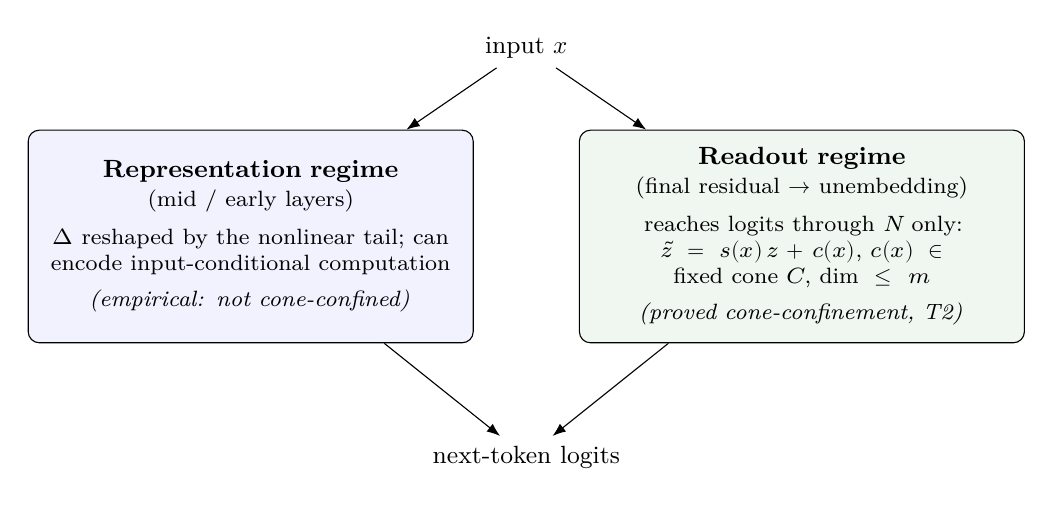
\begin{tikzpicture}[font=\small,>=Latex,
  box/.style={draw,rounded corners,align=center,text width=5.3cm,inner sep=5pt,minimum height=2.7cm}]
  \node (in) at (0,0) {input $x$};
  \node[box,fill=Blue!5] (rep) at (-3.5,-2.4)
    {\textbf{Representation regime}\\[1pt]\footnotesize(mid / early layers)\\[4pt]
     \footnotesize$\Delta$ reshaped by the nonlinear tail; can encode input-conditional computation\\[2pt]
     \footnotesize\emph{(empirical: not cone-confined)}};
  \node[box,fill=ForestGreen!7] (read) at (3.5,-2.4)
    {\textbf{Readout regime}\\[1pt]\footnotesize(final residual $\to$ unembedding)\\[4pt]
     \footnotesize reaches logits through $N$ only: $\tilde z = s(x)\,z + c(x)$, $c(x)\in$ fixed cone $C$, $\dim \le m$\\[2pt]
     \footnotesize\emph{(proved cone-confinement, T2)}};
  \node (out) at (0,-5.2) {next-token logits};
  \draw[->] (in) -- (rep); \draw[->] (in) -- (read);
  \draw[->] (rep) -- (out); \draw[->] (read) -- (out);
\end{tikzpicture}
\caption{\emph{Where the intervention acts decides what it can do.} A representation-regime install (left) is reshaped by the nonlinear tail and can encode input-conditional computation that the logit lens cannot decode (Nadaf, 2026). A readout install (right) reaches the logits through the final norm only, so by T1/T2 its effect is a scalar temperature plus a re-ranking term confined to a fixed $\le m$-dimensional cone chosen before any input. We prove the right-hand confinement; the left-hand non-confinement is cited as empirical.}
\label{fig:regimes}
\end{figure}

We \textbf{do not} claim a formal lattice $G_{\mathrm{read}} \subsetneq G_{\mathrm{repr}}$ between the behaviors realizable by readout installs and by representation-regime (mid-layer) interventions. A general containment in either direction is not proven here: the ``easy'' direction $G_{\mathrm{read}} \subseteq G_{\mathrm{repr}}$ is not obviously true (a fixed mid-layer perturbation pushed through the nonlinear tail need not reproduce an arbitrary final-residual cone bias), so the two classes may be \textbf{incomparable}, not nested. What we state is the \textbf{provable asymmetry}:

\begin{itemize}
\item \textbf{Readout regime (proved):} re-ranking is confined to a fixed $\le m$-dim cone chosen before any input (T2); the re-ranking residual has affine rank $\le m$ (T2$^{\prime}$).
\item \textbf{Representation regime (empirical, not proved here):} existing function-vector results provide empirical evidence for mid/early-layer steering that is \textbf{not well described as a fixed answer-direction bias under the logit lens} --- it steers even where the logit lens cannot decode the answer at any layer (Nadaf, 2026). We do not compute $d(x)$ for those interventions, so we do not claim their residual rank exceeds a comparable readout install's; the formal residual-rank comparison is future work.
\end{itemize}

\emph{Illustrative witness (sketch, explicitly not a theorem).} A single mid-layer additive steer $h_\ell \mapsto h_\ell + \Delta$ induces $\tilde z(x) = U\cdot N(F_{\ell\to L}(h_\ell(x)+\Delta))$ with $F_{\ell\to L}$ nonlinear; on a task where a hidden bit computed by $F_{\ell\to L}$ gates which of two unembedding-incomparable directions the re-ranking takes, $\{d(x)\}$ has affine rank $> 1$ with input-driven selection --- order-2 input-conditional re-ranking, which no $m=1$ readout install achieves. We offer this as an existence illustration consistent with Nadaf (2026); a model-independent separation (a concrete witness \emph{and} the inclusion direction) is left open (\S10).

\emph{Remark (no $\operatorname{col}(U)$ sleight-of-hand).} Every logit vector from any intervention lies in $\operatorname{col}(U)$ trivially (it is $U$ times something), so the separation is \textbf{not} ``readout stays in $\operatorname{col}(U)$, representation leaves it.'' The sharp invariant is the \textbf{fixed cone}: a readout install's re-ranking is a combination of a \emph{pre-fixed} $\le m$-dim direction set, identical across inputs. The representation-side ``not cone-confined'' half is, in this paper, an \textbf{empirical} fact (Nadaf, 2026), not a proof step --- and ``pre-fixed'' means the installed slot set and keys are frozen \emph{before the input}, explicitly excluding context-time / retrieval-augmented slot selection (where the stored set is chosen per query).

\subsection{Corollaries}

Three operational corollaries follow, each matched to evidence in \S7 (tier stated there).

\begin{itemize}
\item \textbf{C1 --- no hard override under bounded correction.} By T2(b), a pair $(\mathrm{target}, \mathrm{prior})$ flips only when $c_{\mathrm{target}}(x) - c_{\mathrm{prior}}(x) > s(x)\cdot[z_{\mathrm{prior}}(x) - z_{\mathrm{target}}(x)]$. For any \textbf{bounded} install (drift-limited per its calibration, so it stays multi-fact-safe), the left side is bounded by the cone geometry, so there exist base gaps large enough that no flip is possible: bounded readout installs are \textbf{not hard overrides}, even with the install direction exactly correct. (Some peaked priors \emph{can} be flipped --- the claim is the absence of a \emph{guarantee} under bounded correction, not that every peaked prior survives. An \emph{unbounded} install can force a target as argmax --- Tier-B any-token, $+20$ nats --- but only by corrupting every other pairwise gap: a blunt overwrite, not a controlled override.) \emph{Evidence (Tier B, \S7):} injecting the oracle-correct value (\texttt{V == lm\_head[target]}, $\cos \approx 1.0$) at the late residual, scaled $\times 1\dots\times 8$, moves the target logit by only \textbf{$+0.016\dots+0.136$} and the model stays on its peaked prior (8/32). The failure is structural, not a wrong-direction problem.

\item \textbf{C2 --- can only \emph{tip} a context-scaffolded near-balanced decision.} When in-context structure flattens the base gap across the candidate set, a small bias from $C$ selects the target --- and the composition is performed by the \textbf{visible context, not by the injected module}, consistent with T2. \emph{Evidence (Tier B, \S7):} a composition surface with a \textbf{visible} runtime operand reaches 272/272 at the \textbf{oracle / exact-captured-per-m delta} --- the \emph{upper bound} (controls: no-module 0.2684, wrong-delta 0.0551, so the lift is real and bridge-independent). But the \textbf{learned hidden route on the same surface reaches only 189/272 = 0.695 and fails its pre-registered gate}, and that residual is itself K=4-codebook regression error, \emph{not} module recovery --- so C2's support is the in-context scaffolding plus the controls, \textbf{not} any claim that the module \emph{recovered} the operand. A separate residual-injection arm reaches 32/32 \textbf{only when the bridge$\to$status table is visible in context}, with the no-bridge floor at 7/32.

\item \textbf{C3 --- cannot \emph{compute} a hidden intermediate (conditional).} A readout install cannot create a new answer direction or compute a routing variable (T2/T2$^{\prime}$); it can route to a hidden bridge \textbf{only if} the addressing query already exposes it. So multi-hop chaining fails whenever the bridge is not linearly available to the addressor --- an empirical property of the surface, not a T2 consequence alone (see \S4.3). \emph{Evidence (Tier B, \S7), across three families:} installing the captured first-hop delta and forcing a second decode fails to chain --- on \textbf{Llama-3.1-8B} the strongest single-pass multi-hop cell is \textbf{0.183 vs a 0.40 bar} (n=372 MQuAKE-CF chains; McNemar canon-vs-control p = $2.15\times10^{-20}$), with the honest caveat that this surface installs at the \emph{subject} positions and Phase-2 re-encodes the bridge, so it is a \textbf{locus-confounded near-miss}, not a pure final-residual wall; a \textbf{Llama$\to$Mistral cross-host} install-then-continue gate reaches \textbf{0.120 vs a 0.70 bar} (n=50). A mid-layer ``read'' --- on a small \emph{from-scratch CCA substrate} (toy; artifacts off-repo) --- is bias-equivalent (cosine 0.9918) with below-chance composition (2/16 $<$ 0.25) and payload-swap 0/3. A directly-built \emph{hidden} second-hop surface failed its own positive control (8/32 at base rate) and is reported in \S7 as a failed construction, not as a clean wall demonstration.
\end{itemize}

\section{Capacity of the readout regime (empirical observations)}

Co-installing $\{(t_i,K_i,\alpha_i)\}$ gives, at a decision, the combined re-ranking term $\sum_i b_i(x)\, u_{t_i}$. Two \emph{distinct} geometries govern capacity and must not be conflated:

\begin{itemize}
\item \textbf{Across decisions — key-disjointness.} When at most one module is addressed per decision ($a_i \approx 0$ for non-matching modules), installs are \textbf{additive and non-interfering}. Empirically, co-loaded single-fact modules give \textbf{bit-exact} output ($\Delta = 0$) and idempotent load/unload with \texttt{Δppl=0} against the unmodified model: 43 real-Wikipedia knowledge bases holding \textasciitilde{}2,580 facts, per-KB co-load $\Delta = +0.00$ pp at the 95th percentile, plus an N=100 synthetic co-load. The cross-decision capacity is, for practical purposes, unbounded \emph{given key-disjointness} — this is a property of the keys, not a theorem about the values. (We say ``tens of co-loaded modules holding thousands of facts,'' not ``thousands of modules,'' to match the measured records.)

\item \textbf{Within a decision — value-cone degeneracy.} Softmax is winner-take-all and the \texttt{lm\_head}-row Gram is far from orthogonal, so the number of independently \emph{co-winnable} targets at one decision is small — empirically \textbf{$\approx 2$}. (Source: a K-target packet probe — at K=2, \textbf{at least one of the two installed targets wins the argmax} on all three architectures (Llama 14/15, Mistral 15/15, Qwen 11/15) against a \textbf{substrate-clean random control} (zero hits across 1,600 random control packets); but the \textbf{strict both-win rate is only 3/15 (Llama) / 2/15 (Mistral) / 1/15 (Qwen)} — the readout is \textbf{winner-take-all} (K-way competition), \emph{not} additive co-installation, and K$\ge$3 collapses. Corroborated by an in-context K-readability degradation 93.75\% (K=4) $\to$ 64\% (K=6) $\to$ 53\% (K=8). We report $\approx 2$ as the clean single-decision argmax ceiling.)
\end{itemize}

\textbf{Reconciling the two capacity figures.} The single-decision argmax ceiling ($\approx 2$) and the \textbf{entropy-effective rank of the output projection ($\approx 917.83 \approx 918$} on Qwen2.5-7B; stable rank $\approx 10.04$, participation ratio $\approx 93.45$, mean $|\cos|$ 0.082, p95 0.233) are different quantities, not a contradiction: $\approx 918$ is a \textbf{spectral property of the output projection $U$ alone} (an entropy-effective rank), \emph{not} an operational capacity — it bounds nothing we prove here; the across-decision capacity is governed by \textbf{key-disjointness} (above), not by $U$'s spectrum, while $\approx 2$ counts how many targets can \emph{co-win within one} decision. Both are empirical observations. The clean derivation of the $\approx 2$ ceiling from the Gram structure of $C$ plus softmax saturation, and any exact link to the effective rank, is left for future work. We summarize: \emph{capacity is effectively unbounded across key-disjoint decisions and $\approx 2$ within a single decision — both empirical observations, not a proved bound.}

\section{The basis-privilege probes (falsification battery)}

T1 is \emph{exact} because the stored value is the \texttt{lm\_head} row (under direct addition; \S 2). Seven falsification probes isolate that the privileged write direction is specifically the \textbf{output-projection row of the target token}. Each replaces or perturbs the installed value and asks whether the install still \textbf{flips the argmax}; at the flip level, only the genuine \texttt{lm\_head} row survives (with one important off-axis caveat stated at the end of this section). Figures below are on Qwen2.5-7B unless noted. These probes support the \emph{mechanism} reading of T1 — that the privileged write direction is the unembedding row — and are not required for the T2 bound, which is purely algebraic.

\begin{table}[ht]\centering\footnotesize
\begin{tabular}{c p{2.6cm} p{3.6cm} p{4.6cm}}
\toprule
\# & Probe & Control it kills & Measured outcome \\
\midrule
1 & Row-specific & random vector @ matched norm & $\approx 0$ recall; only the true row works \\
2 & Subspace & random vector in top-k right-singular subspace, k$\in\{$10,100,918$\}$ & $\approx 0$ recall, \textbf{no monotone ramp in k} \\
3 & Token-identity & \texttt{lm\_head[(t+offset) mod V]} & \textbf{zero} canonical-target recall (biases the offset token) \\
4 & Output-projection & \texttt{embed\_tokens[t]} (input embedding), untied model & \textbf{zero} recall — privilege is the \emph{output} projection \\
5 & Layer-stability & earlier/later late layers & random-A $\approx 0$ at every layer; canonical shows a sharp \textasciitilde{}4$\times$ single-layer jump at the operating layer \\
6 & Magnitude & row-norm correlation & recall $\perp$ row norm: Pearson r $\approx 0.094$, Spearman $\rho \approx 0.167$ (norms span 0.52--0.87) \\
7 & Effective-rank capacity & --- & mean $|\cos|$ 0.082, median 0.061, p95 0.233; stable rank $\approx 10.04$; participation ratio $\approx 93.45$; \textbf{entropy effective rank $\approx 917.83$ ($\approx 918$)}; condition \# $\approx 2.2\times 10^{6}$ \\
\bottomrule
\end{tabular}
\end{table}

\textbf{Cross-family.} The $0.940\to 0.000$ paraphrased-recall collapse under random-A reproduces on Qwen2.5-7B (L27), Llama-3.1-8B (L30), and Mistral-7B-v0.3 (L30); the strong-form privilege is further confirmed on \textbf{untied-embedding} Pythia-1.4B and Pythia-12B (canonical +14.07/+14.08 nats, 10/10 flips, vs random-A +0.37/+0.31; 38$\times$/45$\times$), i.e. 5 architectures / 4 families, 2 verifiably untied. The \textbf{orthogonal-A control} — projecting the \texttt{lm\_head[t]} component out and renorming — is a \emph{pre-registered 4-architecture (Pythia-1.4B / Qwen-7B / Llama-8B / Mistral-7B), 5-seed, cosine-dosage falsification}: it collapses the effect to $\approx$random-A on \textbf{4/4 archs} (orth/canonical ratio: Pythia 1.2\%, Mistral 5.8\%, Llama 18\%, Qwen 38\%), evidence that the privilege rests on the unembedding-readout geometry, i.e. it is exactly the T1 mechanism and not a residual-stream-internal computation.

\textbf{Off-axis caveat (the honest scope of ``only \texttt{lm\_head} survives'').} The probes establish privilege \emph{at the argmax-flip level}: the orthogonal-A install never flips the target (0/10), and flips track $\cos(A, \texttt{lm\_head[t]})$. They do \textbf{not} claim a wrong direction moves the target logit by zero. On instruction-tuned, chat-templated models a \textbf{norm-matched random install} lifts the target logit by a non-trivial amount at large scale ($\approx +7$ nats Qwen, +2.7 Llama, +1 Mistral at $\times 4$; $\approx 0$ on base Pythia), and the cosine-dosage is \textbf{non-monotone on Llama} ($\cos=0.7 \to +20.4$ nats \emph{exceeds} canonical $\cos=1.0 \to +13.9$). This is a residual \emph{attractor}, not a basis privilege — it decomposes as $\Delta\log p \approx \operatorname{DLA}(\cos) + \operatorname{Attractor}(\sqrt{1-\cos^2})$, and the orthogonal-A control rules out a non-DLA mechanism on all 4 archs. We therefore describe $A = \texttt{lm\_head[t]}$ as the \textbf{maximum-readout-coupling deployment direction} (it owns the argmax flip), \textbf{not} as a ``discovered mechanism.''

\begin{figure}[ht]\centering
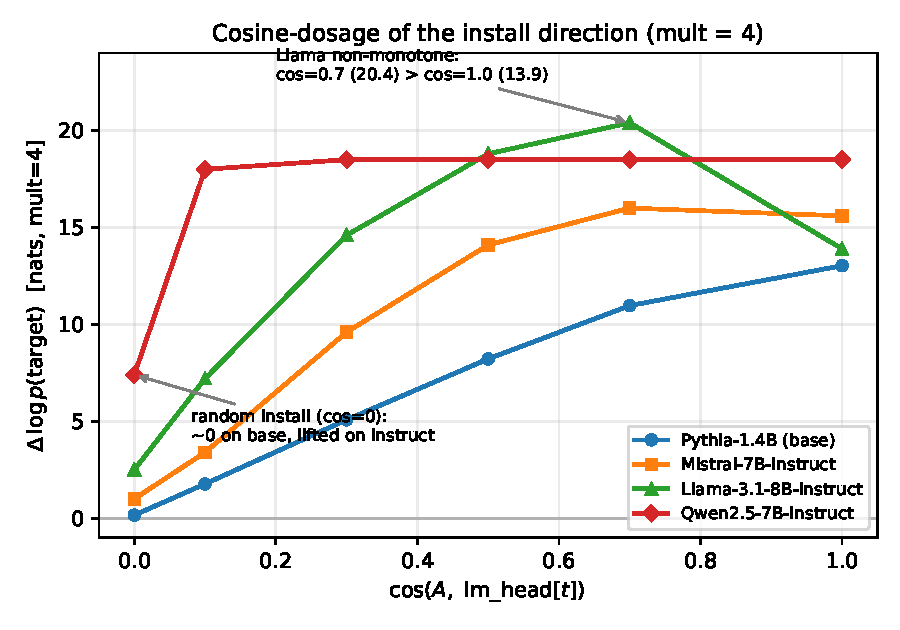
\includegraphics[width=0.80\linewidth]{fig_attractor.pdf}
\caption{\emph{Cosine-dosage of the install direction (norm \texttt{mult = 4}; medians over seeds; Appendix~B.9).} $\Delta \log p$(target) vs $\cos(A, \texttt{lm\_head[t]})$, with $A = c\cdot\hat e_{\mathrm{canon}} + \sqrt{1-c^2}\cdot R_\perp$. On the \textbf{base} model (Pythia-1.4B) the lift is $\approx$linear in $\cos$ and $\approx 0$ at $\cos=0$ — direct logit attribution. On \textbf{instruction-tuned, chat-templated} models a norm-matched \emph{random} install ($\cos=0$) already lifts the target (+7.4 Qwen / +2.5 Llama / +1.0 Mistral nats) and \textbf{Llama is non-monotone} ($\cos=0.7 \to +20.4$ \emph{exceeds} canonical $\cos=1.0 \to +13.9$): an off-axis residual attractor, $\Delta\log p \approx \operatorname{DLA}(\cos) + \operatorname{Attractor}(\sqrt{1-\cos^2})$. The orthogonal-A control ($\cos=0$) never flips the argmax on any architecture, so the \emph{argmax-flip} privilege still belongs to \texttt{lm\_head[t]}. (Values: the \S 6 cosine-dosage sweep, medians over seeds.)}
\label{fig:attractor}
\end{figure}

\section{The empirical map (split by regime)}

We separate evidence at the \textbf{final-residual install site} (Tier A --- literally eq.~(1), the final-norm pre-hook, where T1 is exact) from evidence at a \textbf{late-layer install site} (Tier B --- the operating layer L27/L30, with downstream nonlinear blocks still to run). The tiers test different things: Tier A tests the exact closed form, while in Tier B the remaining layers \emph{could} in principle rescue input-conditional computation. The honest reading of Tier B is an \textbf{empirical pattern}, within one site, consistent with the readout-regime limit (T2 does not formally govern late-layer installs --- \S10): tasks that need only a \textbf{bias} succeed (single-token recall, key-disjoint co-load) while tasks that need \textbf{computation or chaining} hit the wall. Mixing the tiers would be a category error; each row states its injection site.

\textbf{What is load-bearing.} The two theorems stand \emph{algebraically} --- no experiment is required to establish T1, T2, or T2$^{\prime}$ (Appendix~A). The closed-form check ($\approx 5\times10^{-6}$) is a sanity test on the algebra, not support for the claim. The corollaries C1--C3 are \emph{supported, not proved}, by the tiered map below; the capacity figures (\S5) are \emph{exploratory} observations. The map exists to show the limit \textbf{binds in practice}, not to carry the theorem.

\begin{table}[ht]
\centering
\footnotesize
\begin{tabular}{p{4.2cm}p{4.0cm}p{4.0cm}}
\toprule
Claim & Rests on & Role of experiment \\
\midrule
T1 (closed form) & Lemmas 1/3/4 (algebra) & sanity check only (max-diff $\approx 5\times10^{-6}$) \\
T2 / T2$^{\prime}$ (cone-confinement; rank $\le m$) & Lemmas 1--4 (algebra) & none --- proved without experiment \\
C1 (no hard override) & T2(b) & supporting (Tier B readout-wall probe) \\
C2 (only tips) & T2 & supporting (Tier A/B scaffolded composition + controls) \\
C3 (cannot compute a hidden var) & T2/T2$^{\prime}$ + surface property (\S4.3) & supporting (Tier B multi-hop bars) \\
Capacity ($\approx 2$ within / additive across) & --- & exploratory observation (no proof) \\
\bottomrule
\end{tabular}
\end{table}

\subsection*{Tier A --- genuine final-residual installs (direct tests of T1/T2)}

\begin{table}[ht]
\centering
\footnotesize
\begin{tabular}{p{3.0cm}p{2.2cm}p{5.6cm}p{1.6cm}}
\toprule
Observation & Injection site & Decisive numbers & Supports \\
\midrule
Closed form \textbf{is} the rank-1 bias & final residual & direct vs predicted max-diff 4.77e-6 (Mistral, $\alpha=24$), 7.15e-6 (Qwen, $\alpha=64$); rank-1 term = median 96.1\% (Mistral; 96.83\% Qwen) of $\lVert b \rVert$, argmax-preserving & T1, T2(c) \\
Behavioral install & final residual & cross-arch: Llama $+24.61$ / Mistral $+20.40$ (n=20) / Qwen $+17.25$ (n=5 smoke) nats, 0 leakage & C2 (tips a propensity) \\
K-target competition & final residual & $\ge$1-of-2 wins: Llama 14/15, Mistral 15/15, Qwen 11/15 (strict both-win 3/2/1 of 15) vs random control 0/1600; winner-take-all, K$\ge$3 collapses & \S5 ($\approx 2$ ceiling) \\
\bottomrule
\end{tabular}
\end{table}

\subsection*{Tier B --- late-layer installs (downstream nonlinearity available; bias-tasks pass, compute-tasks wall)}

{\footnotesize
\begin{longtable}{p{2.7cm}p{1.9cm}p{5.0cm}p{2.6cm}}
\toprule
Observation & Injection site & Decisive numbers & Supports / caveat \\
\midrule
\endhead
Single-token recall, flat prior (\textbf{bias suffices}) & late layer (L27 Qwen / L30 Llama$\cdot$Mistral) & oracle $\rho=1.000$ across \textbf{6 models, 1.5B--72B, 3 families} (Qwen 1.5B/7B/14B/72B, Llama-8B, Mistral-7B), full $\rho$ 0.900--0.953; $\approx$13$\times$/47$\times$ over MEMIT/ROME paraphrased, $\ge$ top-3 RAG with 0 retrieved tokens; gap to oracle = routing, not content & late-site \textbf{positive}: only a bias is needed (cross-scale) \\
Co-load additivity (\textbf{key-disjoint}) & late layer (L27/L30) & 43-KB / $\sim$2{,}580-fact per-KB co-load $\Delta=+0.00$ pp @ p95; \texttt{Δppl=0}; bit-identical no-harm (0/15{,}498 spurious activations over MMLU+GSM8K+HumanEval); idempotent & late-site \textbf{positive}: \S5 additivity, no computation \\
Composition, \textbf{visible} operand & mid-stack (L18/21) & 272/272 at \textbf{oracle/exact-delta} (upper bound); learned hidden route 189/272=0.695 \textbf{fails its gate} (K=4-codebook regression, not recovery); controls no-module 0.2684, wrong-delta 0.0551 & C2 (in-context, \textbf{not} module recovery) \\
Residual injection, \textbf{table visible} & late residual & 32/32; no-bridge floor 7/32; swap controls follow injected identity & C2 (near-balanced, visibly scaffolded); positive control passes \\
Any-token install (saturating) & late MLP (L27) & target $+20.00$ nats (saturated), 5/5 flip; random-A $-0.44$ (45$\times$) & T1; an unbounded blunt overwrite, not a C2 tip \\
Oracle-correct content fails to move a peaked logit (bounded) & bank @ readout & $+0.016\dots+0.136$ logit at $\times1\dots\times8$; stays 8/32 & C1 (no override guarantee); single-hop, visible bridge \\
Single-pass multi-hop (Llama-3.1-8B) & first-hop install (subject pos) & 0.183 vs 0.40 bar (n=372, McNemar p=2.15e-20; locus-confounded); Llama$\to$Mistral cross-host 0.120 vs 0.70 (n=50) & C3 (no chaining absent an exposed bridge) \\
Mid-layer ``read'' is bias-equivalent & mid-layer (toy from-scratch CCA substrate) & cosine 0.9918 ($\ge$0.95 kill); combine 2/16 $<$ 0.25 chance; payload-swap 0/3 & C3 (read carries no composable content here) \\
Hidden second-hop surface & hidden module & ceiling 8/32 & failed construction: positive control fails 8/32, so it cannot distinguish a T2 wall from a broken surface; reported as such, \textbf{not} as evidence \\
\bottomrule
\end{longtable}}

\textbf{On the ``matched pair.''} It is tempting to present the visible-table 32/32 and the hidden-hop 8/32 as one controlled before/after. They are \textbf{two different surfaces}, and the hidden-hop run failed its own positive control --- so it cannot by itself separate the T2 wall from a broken surface. The honest exhibits are: \textbf{scaffolded success} = the 272/272 composition (oracle/exact-delta upper bound; clean controls) and the visible-table 32/32 (passing positive control); \textbf{no override} = the readout-wall diagnostic (oracle-correct content, $+0.016\dots+0.136$ logit, single-hop); \textbf{cannot chain} = the single-pass multi-hop bars and the mid-layer-read discriminator. The broken hidden-hop surface is reported as such, not as evidence.

Reframed across the map: the final-residual installs (Tier A) behave exactly as the closed form predicts; and at the late-layer site (Tier B) the same pattern is empirically visible --- tasks needing only a bias (recall, key-disjoint co-load) succeed, while tasks needing computation or chaining (hidden-route composition, single-pass multi-hop) hit the wall.

\section{Related work}

\textbf{The established landscape.} Two long-standing lines of work read and write the residual stream. \emph{Reading:} the logit lens (nostalgebraist, 2020) and tuned lens (Belrose et al., 2023, arXiv:2303.08112) decode hidden states through the unembedding; Geva et al. (2021, arXiv:2012.14913; 2022, arXiv:2203.14680) read FFN layers as key--value memories projected into vocabulary space. \emph{Writing:} activation/representation steering --- function vectors (Todd et al., 2024, arXiv:2310.15213; Hendel et al., 2023, arXiv:2310.15916) and steering vectors (Turner et al., 2023, arXiv:2308.10248; Zou et al., 2023, arXiv:2310.01405; Panickssery et al. / CAA, 2024, arXiv:2312.06681) --- adds directions in the \textbf{representation regime} (mid/early layers), while knowledge editors that \emph{write to weights} via gradient-derived rank-one updates (ROME; Meng et al., 2022, arXiv:2202.05262) perform a persistent weight edit, not an inference-time additive install. The representation-engineering survey (Bartoszcze et al., 2025, arXiv:2502.17601) catalogs \emph{cost-type} risks of steering --- performance degradation, compute, and steerability --- which are resource/quality trade-offs distinct from T2's \emph{structural} limit on what can be computed at all. Against this landscape, we characterize \emph{writing in the readout regime} (the final residual) and prove its ceiling.

\textbf{Closest contemporaneous work (2026).} \emph{Closest mechanism.} Wind (2026), \emph{Prometheus Mind: Retrofitting Memory to Frozen Language Models} (arXiv:2601.15324), \S4.4.3 (``Identity V''), already uses a row of \texttt{lm\_head} as an attention value and states that ``row $i$ of \texttt{lm\_head} is precisely the direction that produces high probability for token $i$,'' injecting $v_{\mathrm{memory}} = \alpha\cdot W_{lm}[\mathrm{token}]/\lVert W_{lm}[\mathrm{token}]\rVert\cdot\lVert h\rVert$ into an attention KV pair at one layer for the first generated token. \textbf{T1's core observation is therefore not new.} Wind has \textbf{no} impossibility result, no falsification-probe family, and no capacity theory; our contribution is T2 (cone-confinement) + the probes + the capacity observations. (Mechanistically Wind injects through attention --- hence through $W_O$ --- vs.\ our direct final-residual install; that is the mechanism axis, while this paper is about the \emph{theory} of the readout regime.)

\emph{Complementary regime.} Nadaf (2026), \emph{Steerable but Not Decodable: Function Vectors Operate Beyond the Logit Lens} (arXiv:2604.02608), shows \textbf{empirically} --- across 12 tasks, 6 models, and 4{,}032 cross-template transfers --- that mid-layer function vectors steer behavior \emph{even where the logit lens cannot decode the answer at any layer}, with FVs that reach $>0.90$ steering accuracy still projecting to incoherent token distributions (``FVs encode computational instructions rather than answer directions''). That is precisely a re-ranking effect whose residual is \textbf{not} a fixed \texttt{lm\_head}-row bias --- the \textbf{representation regime}. Nadaf also reports a model-family divergence (Mistral FVs rewrite intermediate representations; Llama/Gemma produce near-zero logit-lens changes despite successful steering), underscoring that the representation regime's mechanism is \emph{not} the uniform readout-bias our T2 characterizes. We supply the closed-form theory of the \textbf{complementary readout regime} and prove its cone-confinement; cited together, the two describe the two-regime picture of \S1/\S4.4.

\emph{Architecture and empirical axes.} \emph{WriteSAE: Sparse Autoencoders for Recurrent State} (Young, 2026, arXiv:2605.12770) independently finds an install$\to$logit closed form for the \textbf{recurrent/state-space write site}: on Gated DeltaNet a formula in the forget gate, read query, and \textbf{output embedding} predicts the resulting logit change at $R^2=0.98$ (88.1\% transfer to Mamba-2-370M) --- the SSM analogue of T1, where the output-embedding row again governs the readout, but with no temperature, cone, capacity, or falsification-probe results; it neither scoops T1's transformer-exact form nor T2. Billa (2026, arXiv:2604.15557), the \emph{Linear Accessibility Profile}, is an \textbf{empirical} predictor of \emph{where} a difference-of-means steering vector succeeds (it applies the unembedding to hidden states), with a three-regime accessibility taxonomy --- complementary to, not overlapping, our \emph{structural} bound. The blog essay \emph{The Mechanism of Logit Gap Steering} (toooold.com, 2026-02-09) treats prompt- and activation-steering as one operation via an ``identity-propagator'' view of the residual stream --- an \emph{approximate} late-layer $\approx$ logit-bias equivalence using generic difference-of-means vectors, with \textbf{no} temperature term, \textbf{no} impossibility, and \textbf{no} capacity bound. (Distinct from the similarly-named jailbreak-suffix paper \emph{Logit-Gap Steering}, arXiv:2506.24056, which we do not rely on.) We give the \emph{exact} equivalence tied to \texttt{lm\_head[token]} (which is \emph{why} it is exact), the temperature, the impossibility (T2), and the capacity observations.

\section{Why it matters: the control reading}

T2 is also a control result. A readout install is an \textbf{auditable} control: by T1 its effect is a removable, composable bias plus a ranking-preserving temperature --- unlike fine-tuning or prompting, you can write down exactly what it does (the closed form matches direct computation to $\approx 5\times10^{-6}$) and undo it bit-exactly. (In the no-norm always-on case the bias is literally input-independent; under RMSNorm/LayerNorm with key-addressed attention it is input-modulated through $b_i(x)$ and $s(x)$ but stays confined to the fixed cone --- still closed-form and removable, just not a single constant.) But T2 says exactly what it \emph{cannot} do, prescribing a two-layer division of labor:

\begin{itemize}
\item \textbf{Put in the readout regime} the jobs that only need to \textbf{tip a propensity}: behavior, tone, persona, refusal/anti-targeting, tool-call suppression. These are near-balanced decisions (C2); a fixed cone bias is the right, auditable instrument, and the final-residual evidence (Tier A: the behavioral install) confirms it works there.
\item \textbf{Do not put in the readout regime} any job that needs a \textbf{hard guarantee} --- authorization gates, capability locks, content that must \emph{override} a determined prior or depend on a hidden computed value. By C1/C3 a bounded readout bias offers no override guarantee against a peaked prior and cannot carry a hidden intermediate. Such guarantees require a \textbf{deterministic override outside the model} (a gate that does not depend on the model winning a logit race).
\end{itemize}

Tip in the readout regime; gate deterministically outside it.

\section{Limitations and open work}

\begin{itemize}
\item \textbf{Capacity derivation.} The single-decision $\approx 2$ ceiling is empirical; deriving it from the Gram structure of $C$ and softmax saturation, and relating it exactly to the effective rank ($\approx 918$), is open.
\item \textbf{Late-stack $\leftrightarrow$ final-residual.} The closed form bridges a \emph{single} late install to the final-residual object; the multi-slot late-stack case (Tier B) is empirically consistent but not proven to collapse to eq.~(1). Either restrict load-bearing claims to final-residual installs (Tier A) or prove the reduction.
\item \textbf{The regime distinction is not a lattice.} We prove readout cone-confinement and cite empirical representation-regime computation; a model-independent formal separation (with both a concrete witness and the inclusion direction) is not established and is left open.
\item \textbf{$W_O$ / attention-addressed memories.} Lemma 1's exact Gram-column form and the \S 6 probes assume direct residual addition; the attention-head version stays cone-confined (T2(c)) but its exact bias direction is $U\cdot W_O\cdot U[t]$. A clean treatment of that case would broaden the probe story.
\item \textbf{Breadth.} T1/T2 are architecture-general (final-residual + unembedding only); the empirical map is Qwen-centric with cross-family probe support. Replicating the readout-wall (C1) and the single-pass-chain limit (C3) end-to-end on $\ge 2$ more families is high-value.
\item \textbf{Reproduction.} Forward-only instrumentation on public checkpoints; every parameter needed to re-derive each reported number is specified in \S 3, \S 6, and Appendix~B (see \emph{Reproducibility}, below).
\end{itemize}

\section{Conclusion}

A final-residual additive intervention on a frozen transformer --- of which installing a scaled \texttt{lm\_head} row is the exactly-characterizable case --- acts on every input as $\tilde z(x) = s(x)\cdot z(x) + c(x)$: a positive scalar temperature plus a re-ranking term drawn from a single fixed, low-dimensional set of directions chosen \emph{before any input} (T1, verified to $\approx 5\times10^{-6}$). The content is not the equivalence --- which is known (Wind, 2026) --- but its \textbf{structure}: because the re-ranking directions are fixed before the input and the addressing weights are non-negative, no input can produce a re-ranking direction outside the pre-installed set, however nonlinear the addressor (T2; the measurable form is the affine-rank bound T2$^{\prime}$). This converts a body of empirical phenomena into corollaries --- a bounded install cannot \emph{override} a peaked prior, can only \emph{tip} a context-scaffolded near-balanced decision, and cannot \emph{compute or carry} a hidden intermediate the addressor does not already expose --- and the empirical map shows the limit binds in practice: final-residual installs (Tier A) behave exactly as the closed form predicts, and at the late-layer site (Tier B) the same pattern is empirically visible --- bias-only tasks succeed while computation and chaining hit the wall. The control reading is the payoff: the readout regime is the right, auditable place for jobs that only need to \emph{tip} a propensity, and the wrong place for any hard guarantee, which requires a deterministic override outside the model. The boundary, stated precisely, is the contribution.

\section*{Reproducibility}

Every result uses publicly available instruction-tuned checkpoints (Qwen2.5-\{1.5B,7B,14B,72B\}, Llama-3.1-8B, Mistral-7B-v0.3, Pythia-1.4B/12B) and forward-only instrumentation --- standard forward hooks; no weights are trained or modified. The paper specifies, for each result, everything needed to rebuild it: the exact checkpoint; the install site (final-norm pre-hook vs.\ late-MLP post-hook) and operating layer; the stored value $\alpha\cdot U[t]$ and the relative-norm calibration that sets $\alpha$; the metric; the decoding setting (greedy/argmax at the install position); and the seeds (Appendix~B). T1's closed form is a two-forward-pass identity (B.4); the basis-privilege probes are direct value substitutions (B.9); the capacity and corollary probes are specified in B.6--B.8; the empirical datasets are named where used (MMLU, GSM8K, HumanEval for the no-harm sweep; MQuAKE-CF for the multi-hop chains). Because the construction is forward-only and the parameters are given, each reported number is re-derivable from the public checkpoints and the procedures in \S 3, \S 6, and Appendix~B.

A companion repository --- \textbf{https://github.com/orbitnate/readout-regime} (MIT) --- provides the authentic script and the committed result artifact behind every reported number, plus a model-free check that reproduces the T1 identity in seconds (no model or GPU). The closed-form verification (\S 3), the \texttt{lm\_head} effective-rank measurement (\S 6), and the K-target capacity probe (\S 5) are clone-and-run on a single 7B checkpoint; the larger cross-scale recall and the Tier-B results ship as the original run artifacts with their source scripts. The MIT license covers the code only and grants no patent rights.

\section*{Broader impact}

This is a theoretical and diagnostic contribution about what a frozen model's readout-space controls can and cannot do; it introduces no new capability and uses only public models. Its main practical consequence is safety-positive: the impossibility (T2) tells builders \emph{not} to rely on a readout-space bias for any hard guarantee --- authorization, capability locks, content that must override a determined prior --- and to place such guarantees in a deterministic mechanism outside the model, reserving the readout regime for auditable, removable propensity tips. We note the usual dual-use caveat that any characterization of steering can inform both helpful and harmful steering; the result here narrows rather than expands what residual-space steering can achieve.

\section*{References}

\begin{itemize}
\item \textbf{Bartoszcze, L., Munshi, S., Sukidi, B., Yen, J., Yang, Z., Williams-King, D., Le, L., Asuzu, K., Maple, C.} (2025). \emph{Representation Engineering for Large-Language Models: Survey and Research Challenges.} arXiv:2502.17601.
\item \textbf{Belrose, N., Ostrovsky, I., McKinney, L., Furman, Z., Smith, L., Halawi, D., Biderman, S., Steinhardt, J.} (2023). \emph{Eliciting Latent Predictions from Transformers with the Tuned Lens.} arXiv:2303.08112.
\item \textbf{Billa, J.} (2026). \emph{Predicting Where Steering Vectors Succeed} (the Linear Accessibility Profile). arXiv:2604.15557.
\item \textbf{Geva, M., Schuster, R., Berant, J., Levy, O.} (2021). \emph{Transformer Feed-Forward Layers Are Key-Value Memories.} EMNLP 2021. arXiv:2012.14913.
\item \textbf{Geva, M., Caciularu, A., Wang, K. R., Goldberg, Y.} (2022). \emph{Transformer Feed-Forward Layers Build Predictions by Promoting Concepts in the Vocabulary Space.} EMNLP 2022. arXiv:2203.14680.
\item \textbf{Hendel, R., Geva, M., Globerson, A.} (2023). \emph{In-Context Learning Creates Task Vectors.} Findings of EMNLP 2023. arXiv:2310.15916.
\item \textbf{Meng, K., Bau, D., Andonian, A., Belinkov, Y.} (2022). \emph{Locating and Editing Factual Associations in GPT} (ROME). NeurIPS 2022. arXiv:2202.05262.
\item \textbf{Nadaf, M. S. B.} (2026). \emph{Steerable but Not Decodable: Function Vectors Operate Beyond the Logit Lens.} arXiv:2604.02608.
\item \textbf{nostalgebraist} (2020). \emph{Interpreting GPT: the Logit Lens.} LessWrong, \url{https://www.lesswrong.com/posts/AcKRB8wDpdaN6v6ru/interpreting-gpt-the-logit-lens}
\item \textbf{Panickssery, N., Gabrieli, N., Schulz, J., Tong, M., Hubinger, E., Turner, A. M.} (2024). \emph{Steering Llama 2 via Contrastive Activation Addition.} ACL 2024. arXiv:2312.06681.
\item \textbf{Todd, E., Li, M. L., Sen Sharma, A., Mueller, A., Wallace, B. C., Bau, D.} (2024). \emph{Function Vectors in Large Language Models.} ICLR 2024. arXiv:2310.15213.
\item \textbf{Turner, A. M., Thiergart, L., Leech, G., Udell, D., Vazquez, J. J., Mini, U., MacDiarmid, M.} (2023). \emph{Activation Addition: Steering Language Models Without Optimization.} arXiv:2308.10248.
\item \textbf{Wind, M.} (2026). \emph{Prometheus Mind: Retrofitting Memory to Frozen Language Models.} arXiv:2601.15324.
\item \textbf{Young, J.} (2026). \emph{WriteSAE: Sparse Autoencoders for Recurrent State.} arXiv:2605.12770.
\item \textbf{Zou, A., Phan, L., Chen, S., Campbell, J., et al.} (2023). \emph{Representation Engineering: A Top-Down Approach to AI Transparency.} arXiv:2310.01405.
\item \emph{The Mechanism of Logit Gap Steering: A Unified View of Prompts, Vectors, and Low-Rank Adaptation.} (2026). Blog essay, toooold.com, 2026-02-09.
\item \emph{Logit-Gap Steering} (jailbreak-suffix attack). (2025). arXiv:2506.24056. Cited only to disambiguate from the essay above; not relied upon.
\end{itemize}

\appendix
\section{Proof details}

\textbf{A.1 Lemma 1.} $U(h+\Delta) = z + U\Delta$, $U\Delta = \sum a_i \alpha_i U U[t_i] = \sum a_i \alpha_i g_{t_i}$. \qed

\textbf{A.2 Lemma 2.} $g_{t_i} = U U[t_i] \in \operatorname{col}(U)$. The set $\{\sum_i a_i\alpha_i g_{t_i} : a_i \ge 0\}$ is the convex cone over the \textbf{signed installed generators} $\{\alpha_i g_{t_i}\}$: if all $\alpha_i \ge 0$ it is $\operatorname{cone}\{g_{t_i}\}$; if some $\alpha_i < 0$ it is the cone over those signed generators, whose linear span is contained in $\operatorname{span}\{g_{t_i}\}$ (dimension $\le m$) and equals the full subspace $\operatorname{span}\{g_{t_i}\}$ \textbf{only if} the installed set supplies enough opposite-signed directions. In all cases $\dim \operatorname{span} \le m$. All of $(U,\{t_i\},\{\alpha_i\})$ are fixed before input. \qed

\textbf{A.3 T2(a)/(b).} No-norm always-on: $\tilde z = z + b$, $b = \sum \alpha_i g_{t_i}$ fixed; $\operatorname{softmax}(z+b)_j = p_j e^{b_j}/\sum_k p_k e^{b_k}$ depends on $x$ only through $p(x)$; equal $p \Rightarrow$ equal output. Gap $\tilde z_j-\tilde z_k = s(x)(z_j-z_k)+(c_j(x)-c_k(x))$, $c(x)\in C$ (Lemmas 1/3/4); $s\equiv 1$, $c$ constant in the no-norm always-on case. \qed

\textbf{A.4 T2(c) and T2$^{\prime}$.} By Lemmas 3/4, $\tilde z(x) = s(x)z(x) + c(x)$, $c(x) = \sum_i b_i(x)u_{t_i} \in C$, $\dim \operatorname{span}(C) \le m$, $C$ fixed before input; $s(x)>0$ preserves the ranking of $z(x)$; an attention sink gives $\sum a_i \le 1$, keeping $c(x)\in C$. Hence $d(x) := \tilde z(x)-s(x)z(x) = c(x) \in C$ for all $x$, so the affine dimension of $\{d(x)\}$ is $\le \dim \operatorname{span}(C) \le m$. \qed

\emph{(No \qedsymbol is claimed for any $G_{\mathrm{read}} \subseteq G_{\mathrm{repr}}$ / $\subsetneq$ statement; per \S4.4 the lattice is not asserted.)}

\section{Experimental details}

All experiments use publicly available instruction-tuned checkpoints and standard forward-pass instrumentation (forward hooks); no weights are trained or modified. We describe each measurement in enough detail to reproduce it from the public model alone.

\textbf{B.1 Models.} Qwen2.5-7B-Instruct (28 layers, hidden 3584, vocab 152064, RMSNorm, \texttt{tie\_word\_embeddings=False}); Llama-3.1-8B-Instruct; Mistral-7B-Instruct-v0.3; Pythia-1.4B and Pythia-12B (both with untied input/output embeddings). All use a final RMSNorm followed by the unembedding \texttt{lm\_head}, except where the LayerNorm analysis of Lemma 4 is invoked.

\textbf{B.2 Install sites.} Two sites are used and always reported per result. \emph{(i) Final residual:} a pre-hook on the final normalization layer adds the install vector to the last-position residual immediately before normalization, so it reaches \texttt{lm\_head} through the norm only --- this is the direct-addition object of eq.~(1) (Tier A). \emph{(ii) Late MLP down-projection:} a post-hook on a selected layer's MLP down-projection adds the install to that layer's output, after which the remaining blocks run normally (Tier B). The operating layer for (ii) is the layer maximizing the basis-privilege gap of \S6 (e.g. L27 on Qwen, L30 on Llama/Mistral).

\textbf{B.3 Install value and scale.} The stored value is $\alpha\cdot U[t]$, the scaled \texttt{lm\_head} row of target token $t$; for the K-target and edit constructions it is a sum/difference of such rows. $\alpha$ is set by a relative-norm calibration (so the added vector's norm is a fixed fraction of the host residual norm at the install position); the per-model $\alpha$ operating points reported in \S7 are stated inline with each result (e.g. the any-token and behavioral installs use the saturating regime).

\textbf{B.4 Closed-form verification (Lemma 3, T1).} For random prompts, we collect the last-position final-layer residual $h$, compute the predicted bias $b_{\mathrm{pred}} = (\alpha/r')\cdot u_t + ((r-r')/(r\cdot r'))\cdot U(\gamma\odot h)$ (with $r,r'$ the RMSNorm denominators before/after install, $u_t = U(\gamma\odot U[t])$), and compare to the \emph{direct} bias $b_{\mathrm{dir}} = \mathrm{logits}(h+\alpha U[t]) - \mathrm{logits}(h)$ obtained by two forward evaluations. We report $\max|b_{\mathrm{pred}} - b_{\mathrm{dir}}|$ over the vocabulary and prompts ($4.77\times10^{-6}$ Mistral at $\alpha=24$, $7.15\times10^{-6}$ Qwen at $\alpha=64$), the fraction of $\lVert b_{\mathrm{dir}}\rVert$ carried by the rank-1 term (median 96.1\% on Mistral, 96.83\% on Qwen), and that the rescale term leaves the argmax unchanged.

\textbf{B.5 A falsification recipe for "is this intervention a readout install?" (T2$^{\prime}$).} Corollary T2$^{\prime}$ is a \emph{proven} bound (Appendix~A.4): a readout install's re-ranking residual at the structural temperature has affine rank $\le m$ by construction, so measuring \emph{that} is tautological and we do not report it as evidence. The useful, falsifiable test runs the other way --- on an intervention of \emph{unknown} type: record the installed logits $\tilde z(x)$ and base logits $z(x)$, form $d(x) = \tilde z(x) - s(x)z(x)$ at the \textbf{structural} temperature $s(x) = r(h(x))/r(\tilde h(x))$ (Lemma 3 --- \textbf{not} a least-squares fit, which would absorb part of $c(x)$ and inflate the rank), and report the affine rank of $\{d(x)\}$. An intervention whose residual rank exceeds its slot count $m$ is \textbf{not} realizable as an m-slot readout install. The natural application --- measuring a mid-layer representation intervention's residual rank to confirm it \emph{exceeds} the readout bound, turning the two-regime separation of \S4.4 from cited into measured --- is left to future work.

\textbf{B.6 Bounded-override probe (C1).} With the install direction set to the oracle-correct \texttt{lm\_head}$[\text{target}]$ (cosine $\approx 1.0$ with the target row), we sweep the scale ($\times1\dots\times8$) at the final-residual install and report the change in the target-token logit and whether the argmax flips; under bounded calibration the target logit moves by only $+0.016\dots+0.136$ and the peaked prior does not flip.

\textbf{B.7 K-target competition (\S5).} We co-install $K$ target rows at one final-residual position and report, per architecture, the \textbf{$\ge$1-of-2-wins} rate and the \textbf{strict both-win} rate at K=2 (and the K$\ge$3 collapse), each against a norm-matched random-row control (zero hits across 1,600 random control packets). The readout is winner-take-all, so co-installed rows compete rather than add.

\textbf{B.8 Co-load additivity (\S5).} We load up to 43 single-fact modules ($\approx$2,580 facts) addressed by disjoint keys, and report the per-module recall solo vs. co-loaded ($\Delta$ at the 95th percentile), the perplexity change against the unmodified model on held-out text (\texttt{Δppl}), and idempotence of load/unload.

\textbf{B.9 Basis-privilege probes (\S6).} Each probe replaces the install value with a control (random vector at matched norm; random vector in the top-k right-singular subspace; wrong-token row; input embedding row; row at a different layer; row scaled across the norm range) and reports recall vs. the genuine \texttt{lm\_head} row. The effective-rank measurement (probe 7) samples vocabulary rows, forms the row matrix, and reports pairwise $|\cos|$ statistics and the singular-spectrum measures (stable rank, participation ratio, entropy effective rank) of the output projection.

\textbf{B.10 Decoding and seeds.} Unless a probe specifies otherwise, scoring is greedy/argmax at the install position; the readout-modifier sensitivity of T1 (argmax-preserving vs. tail-sensitive readouts) is reported separately. Probes that draw random prompts or random control directions fix a seed per run; the reported figures are stable across the seeds used.

\end{document}
